%!TeX root=../wowtop.tex

\ArtChapter[The Man on Putney Hill]{24head}

\lettrine[lines=4,findent=2pt]{I}{} spent that night in the inn that stands at the top of Putney Hill, sleeping in a made bed for the first time since my flight to Leatherhead. I will not tell the needless trouble I had breaking into that house—afterwards I found the front door was on the latch—nor how I ransacked every room for food, until just on the verge of despair, in what seemed to me to be a servant's bedroom, I found a rat-gnawed crust and two tins of pineapple. The place had been already searched and emptied. In the bar I afterwards found some biscuits and sandwiches that had been overlooked. The latter I could not eat, they were too rotten, but the former not only stayed my hunger, but filled my pockets. I lit no lamps, fearing some Martian might come beating that part of London for food in the night. Before I went to bed I had an interval of restlessness, and prowled from window to window, peering out for some sign of these monsters. I slept little. As I lay in bed I found myself thinking consecutively—a thing I do not remember to have done since my last argument with the curate. During all the intervening time my mental condition had been a hurrying succession of vague emotional states or a sort of stupid receptivity. But in the night my brain, reinforced, I suppose, by the food I had eaten, grew clear again, and I thought.

Three things struggled for possession of my mind: the killing of the curate, the whereabouts of the Martians, and the possible fate of my wife. The former gave me no sensation of horror or remorse to recall; I saw it simply as a thing done, a memory infinitely disagreeable but quite without the quality of remorse. I saw myself then as I see myself now, driven step by step towards that hasty blow, the creature of a sequence of accidents leading inevitably to that. I felt no condemnation; yet the memory, static, unprogressive, haunted me. In the silence of the night, with that sense of the nearness of God that sometimes comes into the stillness and the darkness, I stood my trial, my only trial, for that moment of wrath and fear. I retraced every step of our conversation from the moment when I had found him crouching beside me, heedless of my thirst, and pointing to the fire and smoke that streamed up from the ruins of Weybridge. We had been incapable of co-operation—grim chance had taken no heed of that. Had I foreseen, I should have left him at Halliford. But I did not foresee; and crime is to foresee and do. And I set this down as I have set all this story down, as it was. There were no witnesses—all these things I might have concealed. But I set it down, and the reader must form his judgment as he will.

And when, by an effort, I had set aside that picture of a prostrate body, I faced the problem of the Martians and the fate of my wife. For the former I had no data; I could imagine a hundred things, and so, unhappily, I could for the latter. And suddenly that night became terrible. I found myself sitting up in bed, staring at the dark. I found myself praying that the Heat-Ray might have suddenly and painlessly struck her out of being. Since the night of my return from Leatherhead I had not prayed. I had uttered prayers, fetish prayers, had prayed as heathens mutter charms when I was in extremity; but now I prayed indeed, pleading steadfastly and sanely, face to face with the darkness of God. Strange night! Strangest in this, that so soon as dawn had come, I, who had talked with God, crept out of the house like a rat leaving its hiding place—a creature scarcely larger, an inferior animal, a thing that for any passing whim of our masters might be hunted and killed. Perhaps they also prayed confidently to God. Surely, if we have learned nothing else, this war has taught us pity—pity for those witless souls that suffer our dominion.

The morning was bright and fine, and the eastern sky glowed pink, and was fretted with little golden clouds. In the road that runs from the top of Putney Hill to Wimbledon was a number of poor vestiges of the panic torrent that must have poured Londonward on the Sunday night after the fighting began. There was a little two-wheeled cart inscribed with the name of Thomas Lobb, Greengrocer, New Malden, with a smashed wheel and an abandoned tin trunk; there was a straw hat trampled into the now hardened mud, and at the top of West Hill a lot of blood-stained glass about the overturned water trough. My movements were languid, my plans of the vaguest. I had an idea of going to Leatherhead, though I knew that there I had the poorest chance of finding my wife. Certainly, unless death had overtaken them suddenly, my cousins and she would have fled thence; but it seemed to me I might find or learn there whither the Surrey people had fled. I knew I wanted to find my wife, that my heart ached for her and the world of men, but I had no clear idea how the finding might be done. I was also sharply aware now of my intense loneliness. From the corner I went, under cover of a thicket of trees and bushes, to the edge of Wimbledon Common, stretching wide and far.

That dark expanse was lit in patches by yellow gorse and broom; there was no red weed to be seen, and as I prowled, hesitating, on the verge of the open, the sun rose, flooding it all with light and vitality. I came upon a busy swarm of little frogs in a swampy place among the trees. I stopped to look at them, drawing a lesson from their stout resolve to live. And presently, turning suddenly, with an odd feeling of being watched, I beheld something crouching amid a clump of bushes. I stood regarding this. I made a step towards it, and it rose up and became a man armed with a cutlass. I approached him slowly. He stood silent and motionless, regarding me.

As I drew nearer I perceived he was dressed in clothes as dusty and filthy as my own; he looked, indeed, as though he had been dragged through a culvert. Nearer, I distinguished the green slime of ditches mixing with the pale drab of dried clay and shiny, coaly patches. His black hair fell over his eyes, and his face was dark and dirty and sunken, so that at first I did not recognise him. There was a red cut across the lower part of his face.

»Stop!« he cried, when I was within ten yards of him, and I stopped. His voice was hoarse. »Where do you come from?« he said.

I thought, surveying him.

»I come from Mortlake,« I said. »I was buried near the pit the Martians made about their cylinder. I have worked my way out and escaped.«

»There is no food about here,« he said. »This is my country. All this hill down to the river, and back to Clapham, and up to the edge of the common. There is only food for one. Which way are you going?«

I answered slowly.

»I don't know,« I said. »I have been buried in the ruins of a house thirteen or fourteen days. I don't know what has happened.«

He looked at me doubtfully, then started, and looked with a changed expression.

»I've no wish to stop about here,« said I\@. »I think I shall go to Leatherhead, for my wife was there.«

He shot out a pointing finger.

»It is you,« said he; »the man from Woking. And you weren't killed at Weybridge?«

I recognised him at the same moment.

»You are the artilleryman who came into my garden.«

»Good luck!« he said. »We are lucky ones! Fancy \textit{you}!« He put out a hand, and I took it. »I crawled up a drain,« he said. »But they didn't kill everyone. And after they went away I got off towards Walton across the fields. But— It's not sixteen days altogether—and your hair is grey.« He looked over his shoulder suddenly. »Only a rook,« he said. »One gets to know that birds have shadows these days. This is a bit open. Let us crawl under those bushes and talk.«

»Have you seen any Martians?« I said. »Since I crawled out\longdash«

»They've gone away across London,« he said. »I guess they've got a bigger camp there. Of a night, all over there, Hampstead way, the sky is alive with their lights. It's like a great city, and in the glare you can just see them moving. By daylight you can't. But nearer—I haven't seen them\longdash« (he counted on his fingers) »five days. Then I saw a couple across Hammersmith way carrying something big. And the night before last«—he stopped and spoke impressively—»it was just a matter of lights, but it was something up in the air. I believe they've built a flying-machine, and are learning to fly.«

I stopped, on hands and knees, for we had come to the bushes.

»Fly!«

»Yes,« he said, »fly.«

I went on into a little bower, and sat down.

»It is all over with humanity,« I said. »If they can do that they will simply go round the world.«

He nodded.

»They will. But— It will relieve things over here a bit. And besides\longdash« He looked at me. »Aren't you satisfied it \textit{is} up with humanity? I am. We're down; we're beat.«

I stared. Strange as it may seem, I had not arrived at this fact—a fact perfectly obvious so soon as he spoke. I had still held a vague hope; rather, I had kept a lifelong habit of mind. He repeated his words, »We're beat.« They carried absolute conviction.

»It's all over,« he said. »They've lost \textit{one}—just \textit{one}. And they've made their footing good and crippled the greatest power in the world. They've walked over us. The death of that one at Weybridge was an accident. And these are only pioneers. They kept on coming. These green stars—I've seen none these five or six days, but I've no doubt they're falling somewhere every night. Nothing's to be done. We're under! We're beat!«

I made him no answer. I sat staring before me, trying in vain to devise some countervailing thought.

»This isn't a war,« said the artilleryman. »It never was a war, any more than there's war between man and ants.«

Suddenly I recalled the night in the observatory.

»After the tenth shot they fired no more—at least, until the first cylinder came.«

»How do you know?« said the artilleryman. I explained. He thought. »Something wrong with the gun,« he said. »But what if there is? They'll get it right again. And even if there's a delay, how can it alter the end? It's just men and ants. There's the ants builds their cities, live their lives, have wars, revolutions, until the men want them out of the way, and then they go out of the way. That's what we are now—just ants. Only\longdash«

»Yes,« I said.

»We're eatable ants.«

We sat looking at each other.

»And what will they do with us?« I said.

»That's what I've been thinking,« he said; »that's what I've been thinking. After Weybridge I went south—thinking. I saw what was up. Most of the people were hard at it squealing and exciting themselves. But I'm not so fond of squealing. I've been in sight of death once or twice; I'm not an ornamental soldier, and at the best and worst, death—it's just death. And it's the man that keeps on thinking comes through. I saw everyone tracking away south. Says I, »Food won't last this way,« and I turned right back. I went for the Martians like a sparrow goes for man. All round«—he waved a hand to the horizon—»they're starving in heaps, bolting, treading on each other\textellipsis«

He saw my face, and halted awkwardly.

»No doubt lots who had money have gone away to France,« he said. He seemed to hesitate whether to apologise, met my eyes, and went on: »There's food all about here. Canned things in shops; wines, spirits, mineral waters; and the water mains and drains are empty. Well, I was telling you what I was thinking. »Here's intelligent things,« I said, »and it seems they want us for food. First, they'll smash us up—ships, machines, guns, cities, all the order and organisation. All that will go. If we were the size of ants we might pull through. But we're not. It's all too bulky to stop. That's the first certainty.« Eh?«

I assented.

»It is; I've thought it out. Very well, then—next; at present we're caught as we're wanted. A Martian has only to go a few miles to get a crowd on the run. And I saw one, one day, out by Wandsworth, picking houses to pieces and routing among the wreckage. But they won't keep on doing that. So soon as they've settled all our guns and ships, and smashed our railways, and done all the things they are doing over there, they will begin catching us systematic, picking the best and storing us in cages and things. That's what they will start doing in a bit. Lord! They haven't begun on us yet. Don't you see that?«

»Not begun!« I exclaimed.

»Not begun. All that's happened so far is through our not having the sense to keep quiet—worrying them with guns and such foolery. And losing our heads, and rushing off in crowds to where there wasn't any more safety than where we were. They don't want to bother us yet. They're making their things—making all the things they couldn't bring with them, getting things ready for the rest of their people. Very likely that's why the cylinders have stopped for a bit, for fear of hitting those who are here. And instead of our rushing about blind, on the howl, or getting dynamite on the chance of busting them up, we've got to fix ourselves up according to the new state of affairs. That's how I figure it out. It isn't quite according to what a man wants for his species, but it's about what the facts point to. And that's the principle I acted upon. Cities, nations, civilisation, progress—it's all over. That game's up. We're beat.«

»But if that is so, what is there to live for?«

The artilleryman looked at me for a moment.

»There won't be any more blessed concerts for a million years or so; there won't be any Royal Academy of Arts, and no nice little feeds at restaurants. If it's amusement you're after, I reckon the game is up. If you've got any drawing-room manners or a dislike to eating peas with a knife or dropping aitches, you'd better chuck 'em away. They ain't no further use.«

»You mean\longdash«

»I mean that men like me are going on living—for the sake of the breed. I tell you, I'm grim set on living. And if I'm not mistaken, you'll show what insides \textit{you've} got, too, before long. We aren't going to be exterminated. And I don't mean to be caught either, and tamed and fattened and bred like a thundering ox. Ugh! Fancy those brown creepers!«

»You don't mean to say\longdash«

»I do. I'm going on, under their feet. I've got it planned; I've thought it out. We men are beat. We don't know enough. We've got to learn before we've got a chance. And we've got to live and keep independent while we learn. See! That's what has to be done.«

I stared, astonished, and stirred profoundly by the man's resolution.

»Great God!« cried I\@. »But you are a man indeed!« And suddenly I gripped his hand.

»Eh!« he said, with his eyes shining. »I've thought it out, eh?«

»Go on,« I said.

»Well, those who mean to escape their catching must get ready. I'm getting ready. Mind you, it isn't all of us that are made for wild beasts; and that's what it's got to be. That's why I watched you. I had my doubts. You're slender. I didn't know that it was you, you see, or just how you'd been buried. All these—the sort of people that lived in these houses, and all those damn little clerks that used to live down \textit{that} way—they'd be no good. They haven't any spirit in them—no proud dreams and no proud lusts; and a man who hasn't one or the other—Lord! What is he but funk and precautions? They just used to skedaddle off to work—I've seen hundreds of 'em, bit of breakfast in hand, running wild and shining to catch their little season-ticket train, for fear they'd get dismissed if they didn't; working at businesses they were afraid to take the trouble to understand; skedaddling back for fear they wouldn't be in time for dinner; keeping indoors after dinner for fear of the back streets, and sleeping with the wives they married, not because they wanted them, but because they had a bit of money that would make for safety in their one little miserable skedaddle through the world. Lives insured and a bit invested for fear of accidents. And on Sundays—fear of the hereafter. As if hell was built for rabbits! Well, the Martians will just be a godsend to these. Nice roomy cages, fattening food, careful breeding, no worry. After a week or so chasing about the fields and lands on empty stomachs, they'll come and be caught cheerful. They'll be quite glad after a bit. They'll wonder what people did before there were Martians to take care of them. And the bar loafers, and mashers, and singers—I can imagine them. I can imagine them,« he said, with a sort of sombre gratification. »There'll be any amount of sentiment and religion loose among them. There's hundreds of things I saw with my eyes that I've only begun to see clearly these last few days. There's lots will take things as they are—fat and stupid; and lots will be worried by a sort of feeling that it's all wrong, and that they ought to be doing something. Now whenever things are so that a lot of people feel they ought to be doing something, the weak, and those who go weak with a lot of complicated thinking, always make for a sort of do-nothing religion, very pious and superior, and submit to persecution and the will of the Lord. Very likely you've seen the same thing. It's energy in a gale of funk, and turned clean inside out. These cages will be full of psalms and hymns and piety. And those of a less simple sort will work in a bit of—what is it?—eroticism.«

He paused.

»Very likely these Martians will make pets of some of them; train them to do tricks—who knows?—get sentimental over the pet boy who grew up and had to be killed. And some, maybe, they will train to hunt us.«

»No,« I cried, »that's impossible! No human being\longdash«

»What's the good of going on with such lies?« said the artilleryman. »There's men who'd do it cheerful. What nonsense to pretend there isn't!«

And I succumbed to his conviction.

»If they come after me,« he said; »Lord, if they come after me!« and subsided into a grim meditation.

I sat contemplating these things. I could find nothing to bring against this man's reasoning. In the days before the invasion no one would have questioned my intellectual superiority to his—I, a professed and recognised writer on philosophical themes, and he, a common soldier; and yet he had already formulated a situation that I had scarcely realised.

»What are you doing?« I said presently. »What plans have you made?«

He hesitated.

»Well, it's like this,« he said. »What have we to do? We have to invent a sort of life where men can live and breed, and be sufficiently secure to bring the children up. Yes—wait a bit, and I'll make it clearer what I think ought to be done. The tame ones will go like all tame beasts; in a few generations they'll be big, beautiful, rich-blooded, stupid—rubbish! The risk is that we who keep wild will go savage—degenerate into a sort of big, savage rat\textellipsis You see, how I mean to live is underground. I've been thinking about the drains. Of course those who don't know drains think horrible things; but under this London are miles and miles—hundreds of miles—and a few days rain and London empty will leave them sweet and clean. The main drains are big enough and airy enough for anyone. Then there's cellars, vaults, stores, from which bolting passages may be made to the drains. And the railway tunnels and subways. Eh? You begin to see? And we form a band—able-bodied, clean-minded men. We're not going to pick up any rubbish that drifts in. Weaklings go out again.«

»As you meant me to go?«

»Well—I parleyed, didn't I\@?«

»We won't quarrel about that. Go on.«

»Those who stop obey orders. Able-bodied, clean-minded women we want also—mothers and teachers. No lackadaisical ladies—no blasted rolling eyes. We can't have any weak or silly. Life is real again, and the useless and cumbersome and mischievous have to die. They ought to die. They ought to be willing to die. It's a sort of disloyalty, after all, to live and taint the race. And they can't be happy. Moreover, dying's none so dreadful; it's the funking makes it bad. And in all those places we shall gather. Our district will be London. And we may even be able to keep a watch, and run about in the open when the Martians keep away. Play cricket, perhaps. That's how we shall save the race. Eh? It's a possible thing? But saving the race is nothing in itself. As I say, that's only being rats. It's saving our knowledge and adding to it is the thing. There men like you come in. There's books, there's models. We must make great safe places down deep, and get all the books we can; not novels and poetry swipes, but ideas, science books. That's where men like you come in. We must go to the British Museum and pick all those books through. Especially we must keep up our science—learn more. We must watch these Martians. Some of us must go as spies. When it's all working, perhaps I will. Get caught, I mean. And the great thing is, we must leave the Martians alone. We mustn't even steal. If we get in their way, we clear out. We must show them we mean no harm. Yes, I know. But they're intelligent things, and they won't hunt us down if they have all they want, and think we're just harmless vermin.«

The artilleryman paused and laid a brown hand upon my arm.

»After all, it may not be so much we may have to learn before—Just imagine this: four or five of their fighting machines suddenly starting off—Heat-Rays right and left, and not a Martian in 'em. Not a Martian in 'em, but men—men who have learned the way how. It may be in my time, even—those men. Fancy having one of them lovely things, with its Heat-Ray wide and free! Fancy having it in control! What would it matter if you smashed to smithereens at the end of the run, after a bust like that? I reckon the Martians'll open their beautiful eyes! Can't you see them, man? Can't you see them hurrying, hurrying—puffing and blowing and hooting to their other mechanical affairs? Something out of gear in every case. And swish, bang, rattle, swish! Just as they are fumbling over it, \textit{swish} comes the Heat-Ray, and, behold! man has come back to his own.«

For a while the imaginative daring of the artilleryman, and the tone of assurance and courage he assumed, completely dominated my mind. I believed unhesitatingly both in his forecast of human destiny and in the practicability of his astonishing scheme, and the reader who thinks me susceptible and foolish must contrast his position, reading steadily with all his thoughts about his subject, and mine, crouching fearfully in the bushes and listening, distracted by apprehension. We talked in this manner through the early morning time, and later crept out of the bushes, and, after scanning the sky for Martians, hurried precipitately to the house on Putney Hill where he had made his lair. It was the coal cellar of the place, and when I saw the work he had spent a week upon—it was a burrow scarcely ten yards long, which he designed to reach to the main drain on Putney Hill—I had my first inkling of the gulf between his dreams and his powers. Such a hole I could have dug in a day. But I believed in him sufficiently to work with him all that morning until past midday at his digging. We had a garden barrow and shot the earth we removed against the kitchen range. We refreshed ourselves with a tin of mock-turtle soup and wine from the neighbouring pantry. I found a curious relief from the aching strangeness of the world in this steady labour. As we worked, I turned his project over in my mind, and presently objections and doubts began to arise; but I worked there all the morning, so glad was I to find myself with a purpose again. After working an hour I began to speculate on the distance one had to go before the cloaca was reached, the chances we had of missing it altogether. My immediate trouble was why we should dig this long tunnel, when it was possible to get into the drain at once down one of the manholes, and work back to the house. It seemed to me, too, that the house was inconveniently chosen, and required a needless length of tunnel. And just as I was beginning to face these things, the artilleryman stopped digging, and looked at me.

% \begin{figure}[tbp]
% \centering
% 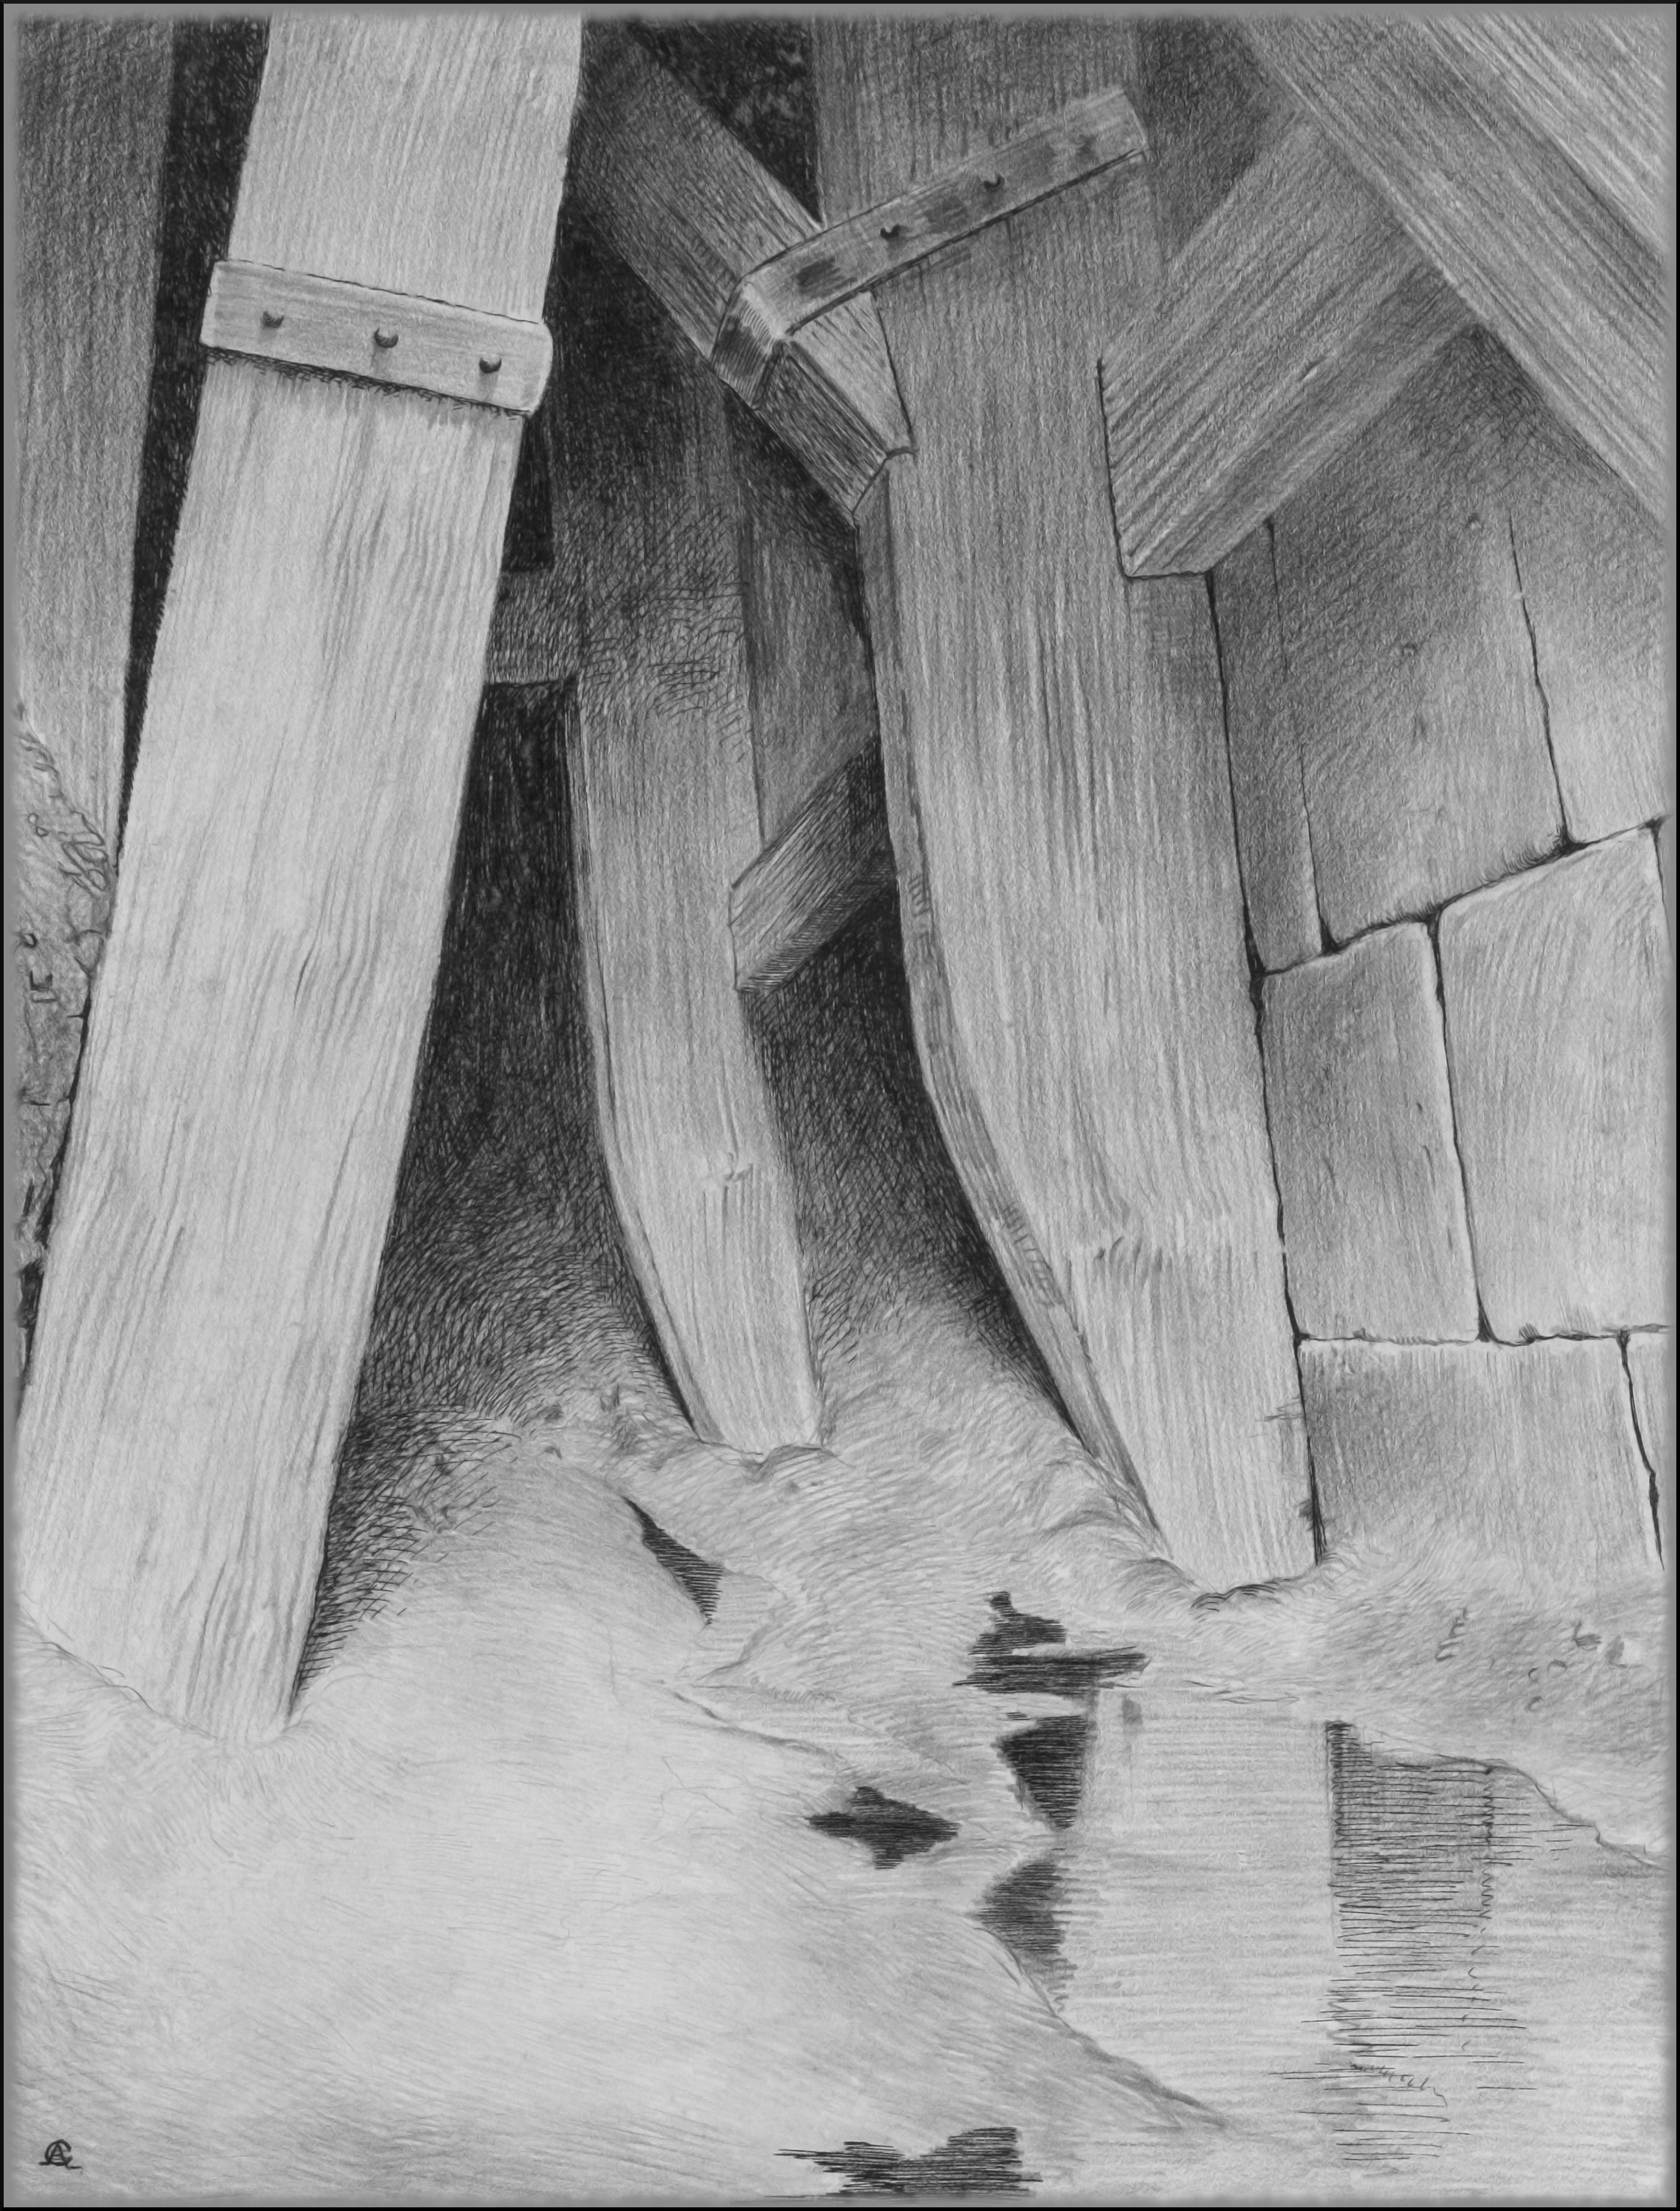
\includegraphics[width=\linewidth]{24drains}
% \caption{A burrow scarcely ten yards long}
% \end{figure}

\begin{letter}
	\begin{bwbigpic}
		[1.2] 
		{24drains} 
		{A burrow scarcely ten yards long} 
	\end{bwbigpic}
\end{letter}
\begin{a4}
	\begin{bwbigpic}
		[1.1] 
		{24drains} 
		{A burrow scarcely ten yards long} 
	\end{bwbigpic}

\end{a4}


»We're working well,« he said. He put down his spade. »Let us knock off a bit« he said. »I think it's time we reconnoitred from the roof of the house.«

I was for going on, and after a little hesitation he resumed his spade; and then suddenly I was struck by a thought. I stopped, and so did he at once.

»Why were you walking about the common,« I said, »instead of being here?«

»Taking the air,« he said. »I was coming back. It's safer by night.«

»But the work?«

»Oh, one can't always work,« he said, and in a flash I saw the man plain. He hesitated, holding his spade. »We ought to reconnoitre now,« he said, »because if any come near they may hear the spades and drop upon us unawares.«

\begin{figure}[tb]
\centering
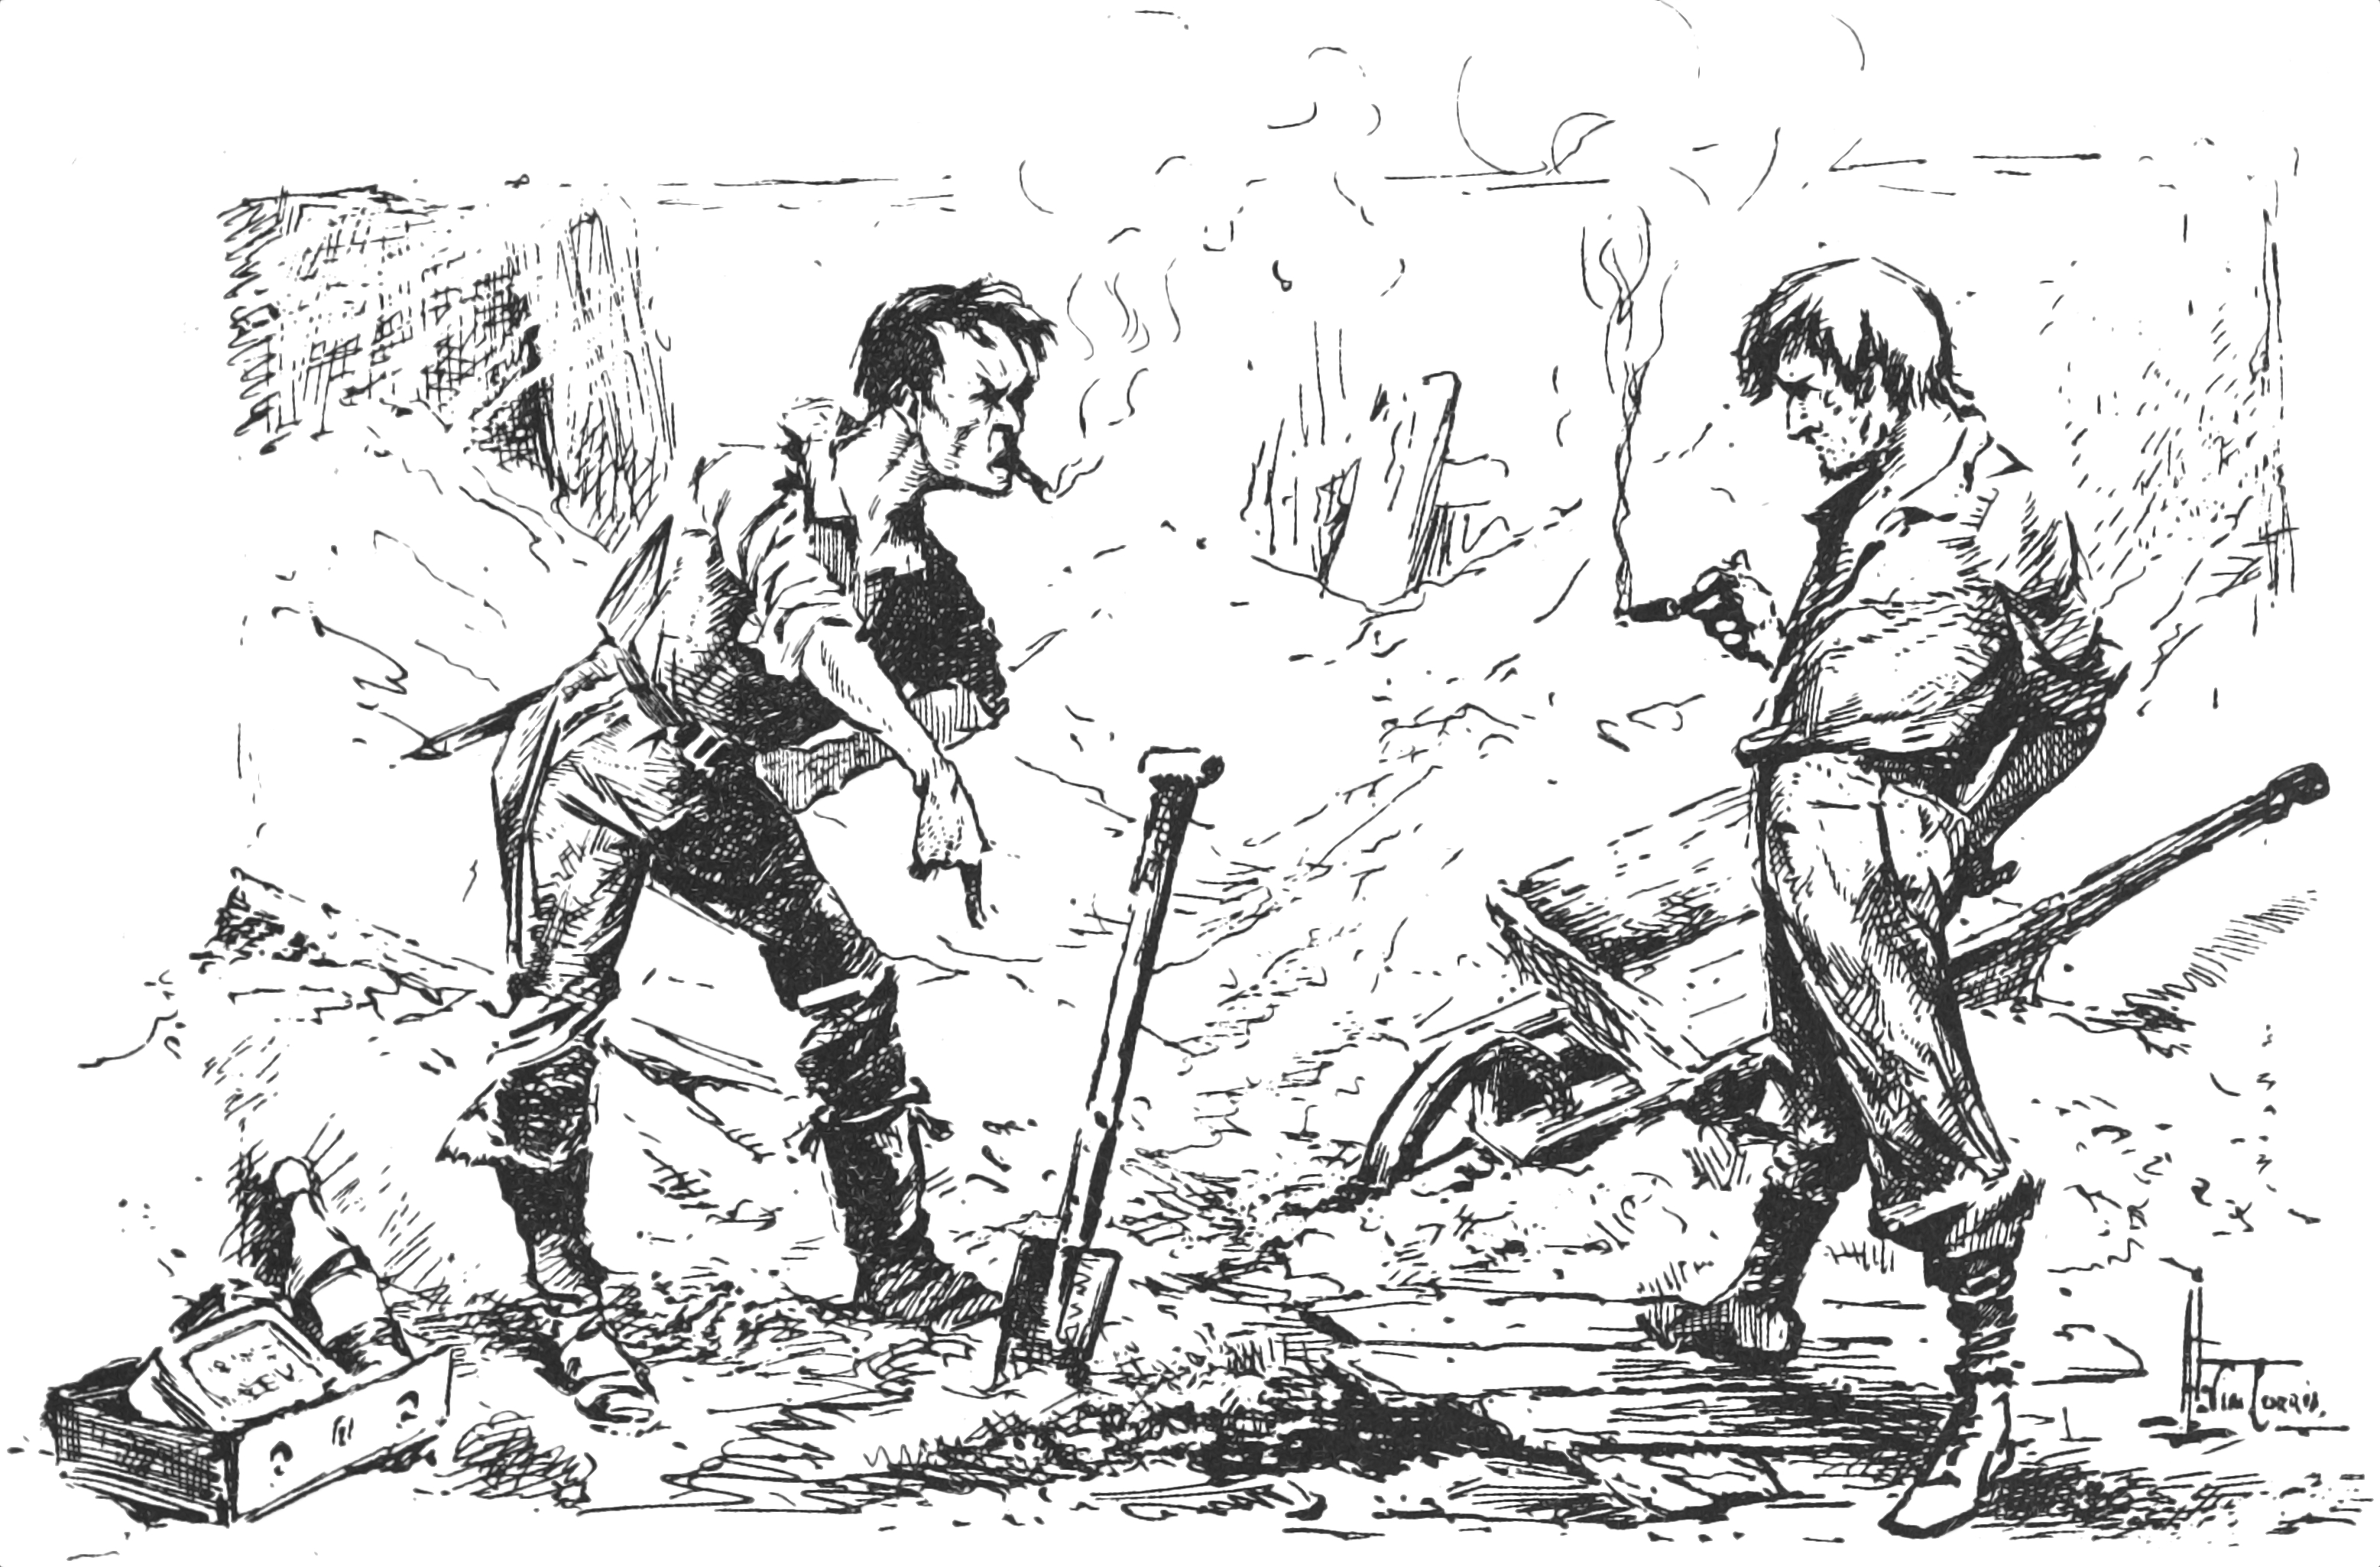
\includegraphics[width=\linewidth]{24argument1}
\end{figure}

I was no longer disposed to object. We went together to the roof and stood on a ladder peeping out of the roof door. No Martians were to be seen, and we ventured out on the tiles, and slipped down under shelter of the parapet.

From this position a shrubbery hid the greater portion of Putney, but we could see the river below, a bubbly mass of red weed, and the low parts of Lambeth flooded and red. The red creeper swarmed up the trees about the old palace, and their branches stretched gaunt and dead, and set with shrivelled leaves, from amid its clusters. It was strange how entirely dependent both these things were upon flowing water for their propagation. About us neither had gained a footing; laburnums, pink mays, snowballs, and trees of arbor-vitae, rose out of laurels and hydrangeas, green and brilliant into the sunlight. Beyond Kensington dense smoke was rising, and that and a blue haze hid the northward hills.

The artilleryman began to tell me of the sort of people who still remained in London.

»One night last week,« he said, »some fools got the electric light in order, and there was all Regent Street and the Circus ablaze, crowded with painted and ragged drunkards, men and women, dancing and shouting till dawn. A man who was there told me. And as the day came they became aware of a fighting-machine standing near by the Langham and looking down at them. Heaven knows how long he had been there. It must have given some of them a nasty turn. He came down the road towards them, and picked up nearly a hundred too drunk or frightened to run away.«


\begin{letter}
	\begin{bwbigpic}
		[1.2] 
		{24circusablaze} 
		{They became aware of a fighting-machine looking down at them} 
		[A fighting-machine looking down at them]
	\end{bwbigpic}
\end{letter}
\begin{a4}
	\begin{bwbigpic}
		[1.1] 
		{24circusablaze} 
		{They became aware of a fighting-machine looking down at them} 
		[A fighting-machine looking down at them]
	\end{bwbigpic}
\end{a4}

Grotesque gleam of a time no history will ever fully describe!

% \begin{wrapfigure}{O}{0.5\textwidth}
% \centering
% 
\includegraphics[width=0.5\textwidth]{24argument2}
% \end{wrapfigure}

\begin{figure}[tb]
	\centering
	
\includegraphics[width=\textwidth]{24argument2}
	%\captionlistentry{Tailpiece to Chapter \thechapter}
\end{figure}

From that, in answer to my questions, he came round to his grandiose plans again. He grew enthusiastic. He talked so eloquently of the possibility of capturing a fighting-machine that I more than half believed in him again. But now that I was beginning to understand something of his quality, I could divine the stress he laid on doing nothing precipitately. And I noted that now there was no question that he personally was to capture and fight the great machine.

After a time we went down to the cellar. Neither of us seemed disposed to resume digging, and when he suggested a meal, I was nothing loath. He became suddenly very generous, and when we had eaten he went away and returned with some excellent cigars. We lit these, and his optimism glowed. He was inclined to regard my coming as a great occasion.

»There's some champagne in the cellar,« he said.

»We can dig better on this Thames-side burgundy,« said I\@.

»No,« said he; »I am host today. Champagne! Great God! We've a heavy enough task before us! Let us take a rest and gather strength while we may. Look at these blistered hands!«

And pursuant to this idea of a holiday, he insisted upon playing cards after we had eaten. He taught me euchre, and after dividing London between us, I taking the northern side and he the southern, we played for parish points. Grotesque and foolish as this will seem to the sober reader, it is absolutely true, and what is more remarkable, I found the card game and several others we played extremely interesting.



Strange mind of man! that, with our species upon the edge of extermination or appalling degradation, with no clear prospect before us but the chance of a horrible death, we could sit following the chance of this painted pasteboard, and playing the »joker« with vivid delight. Afterwards he taught me poker, and I beat him at three tough chess games. When dark came we decided to take the risk, and lit a lamp.

After an interminable string of games, we supped, and the artilleryman finished the champagne. We went on smoking the cigars. He was no longer the energetic regenerator of his species I had encountered in the morning. He was still optimistic, but it was a less kinetic, a more thoughtful optimism. I remember he wound up with my health, proposed in a speech of small variety and considerable intermittence. I took a cigar, and went upstairs to look at the lights of which he had spoken that blazed so greenly along the Highgate hills.



At first I stared unintelligently across the London valley. The northern hills were shrouded in darkness; the fires near Kensington glowed redly, and now and then an orange-red tongue of flame flashed up and vanished in the deep blue night. All the rest of London was black. Then, nearer, I perceived a strange light, a pale, violet-purple fluorescent glow, quivering under the night breeze. For a space I could not understand it, and then I knew that it must be the red weed from which this faint irradiation proceeded. With that realisation my dormant sense of wonder, my sense of the proportion of things, awoke again. I glanced from that to Mars, red and clear, glowing high in the west, and then gazed long and earnestly at the darkness of Hampstead and Highgate.

I remained a very long time upon the roof, wondering at the grotesque changes of the day. I recalled my mental states from the midnight prayer to the foolish card-playing. I had a violent revulsion of feeling. I remember I flung away the cigar with a certain wasteful symbolism. My folly came to me with glaring exaggeration. I seemed a traitor to my wife and to my kind; I was filled with remorse. I resolved to leave this strange undisciplined dreamer of great things to his drink and gluttony, and to go on into London. There, it seemed to me, I had the best chance of learning what the Martians and my fellowmen were doing. I was still upon the roof when the late moon rose.

% \begin{letter}
	% \begin{figure}[b!]
		% \centering
		% 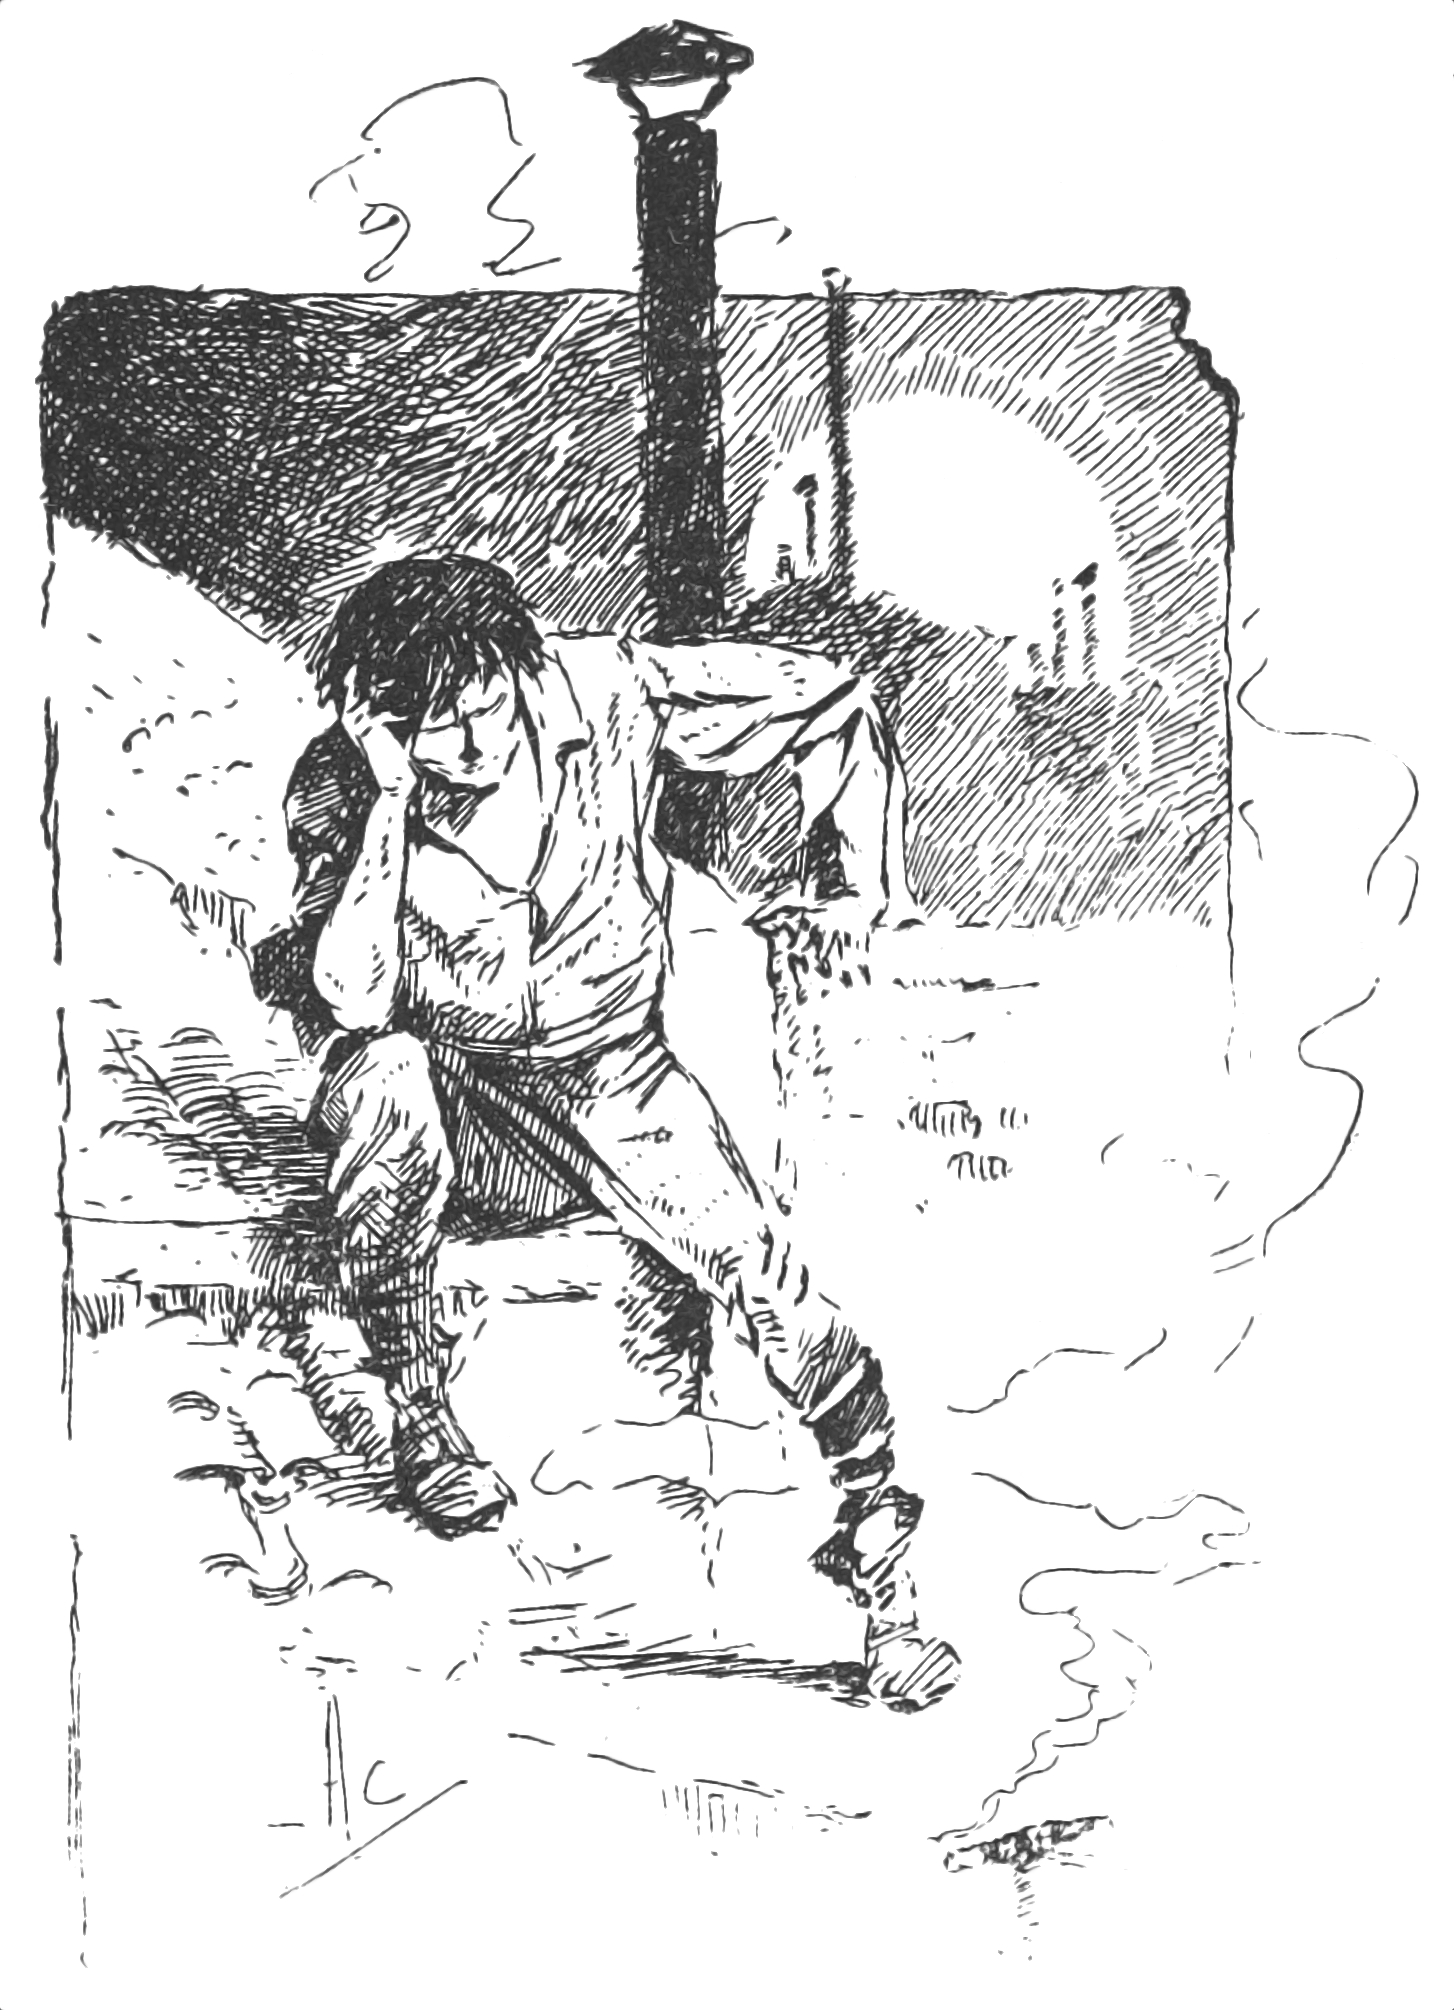
\includegraphics[width=0.7\textwidth]{24tailpiece}
		% %\captionlistentry{Tailpiece to Chapter \thechapter}
	% \end{figure}
% \end{letter}

\begin{a4}
	\begin{tikzpicture}[remember picture, overlay]  
		\node (tailpiece) at ($(current page.south)+(0cm,7cm)$) {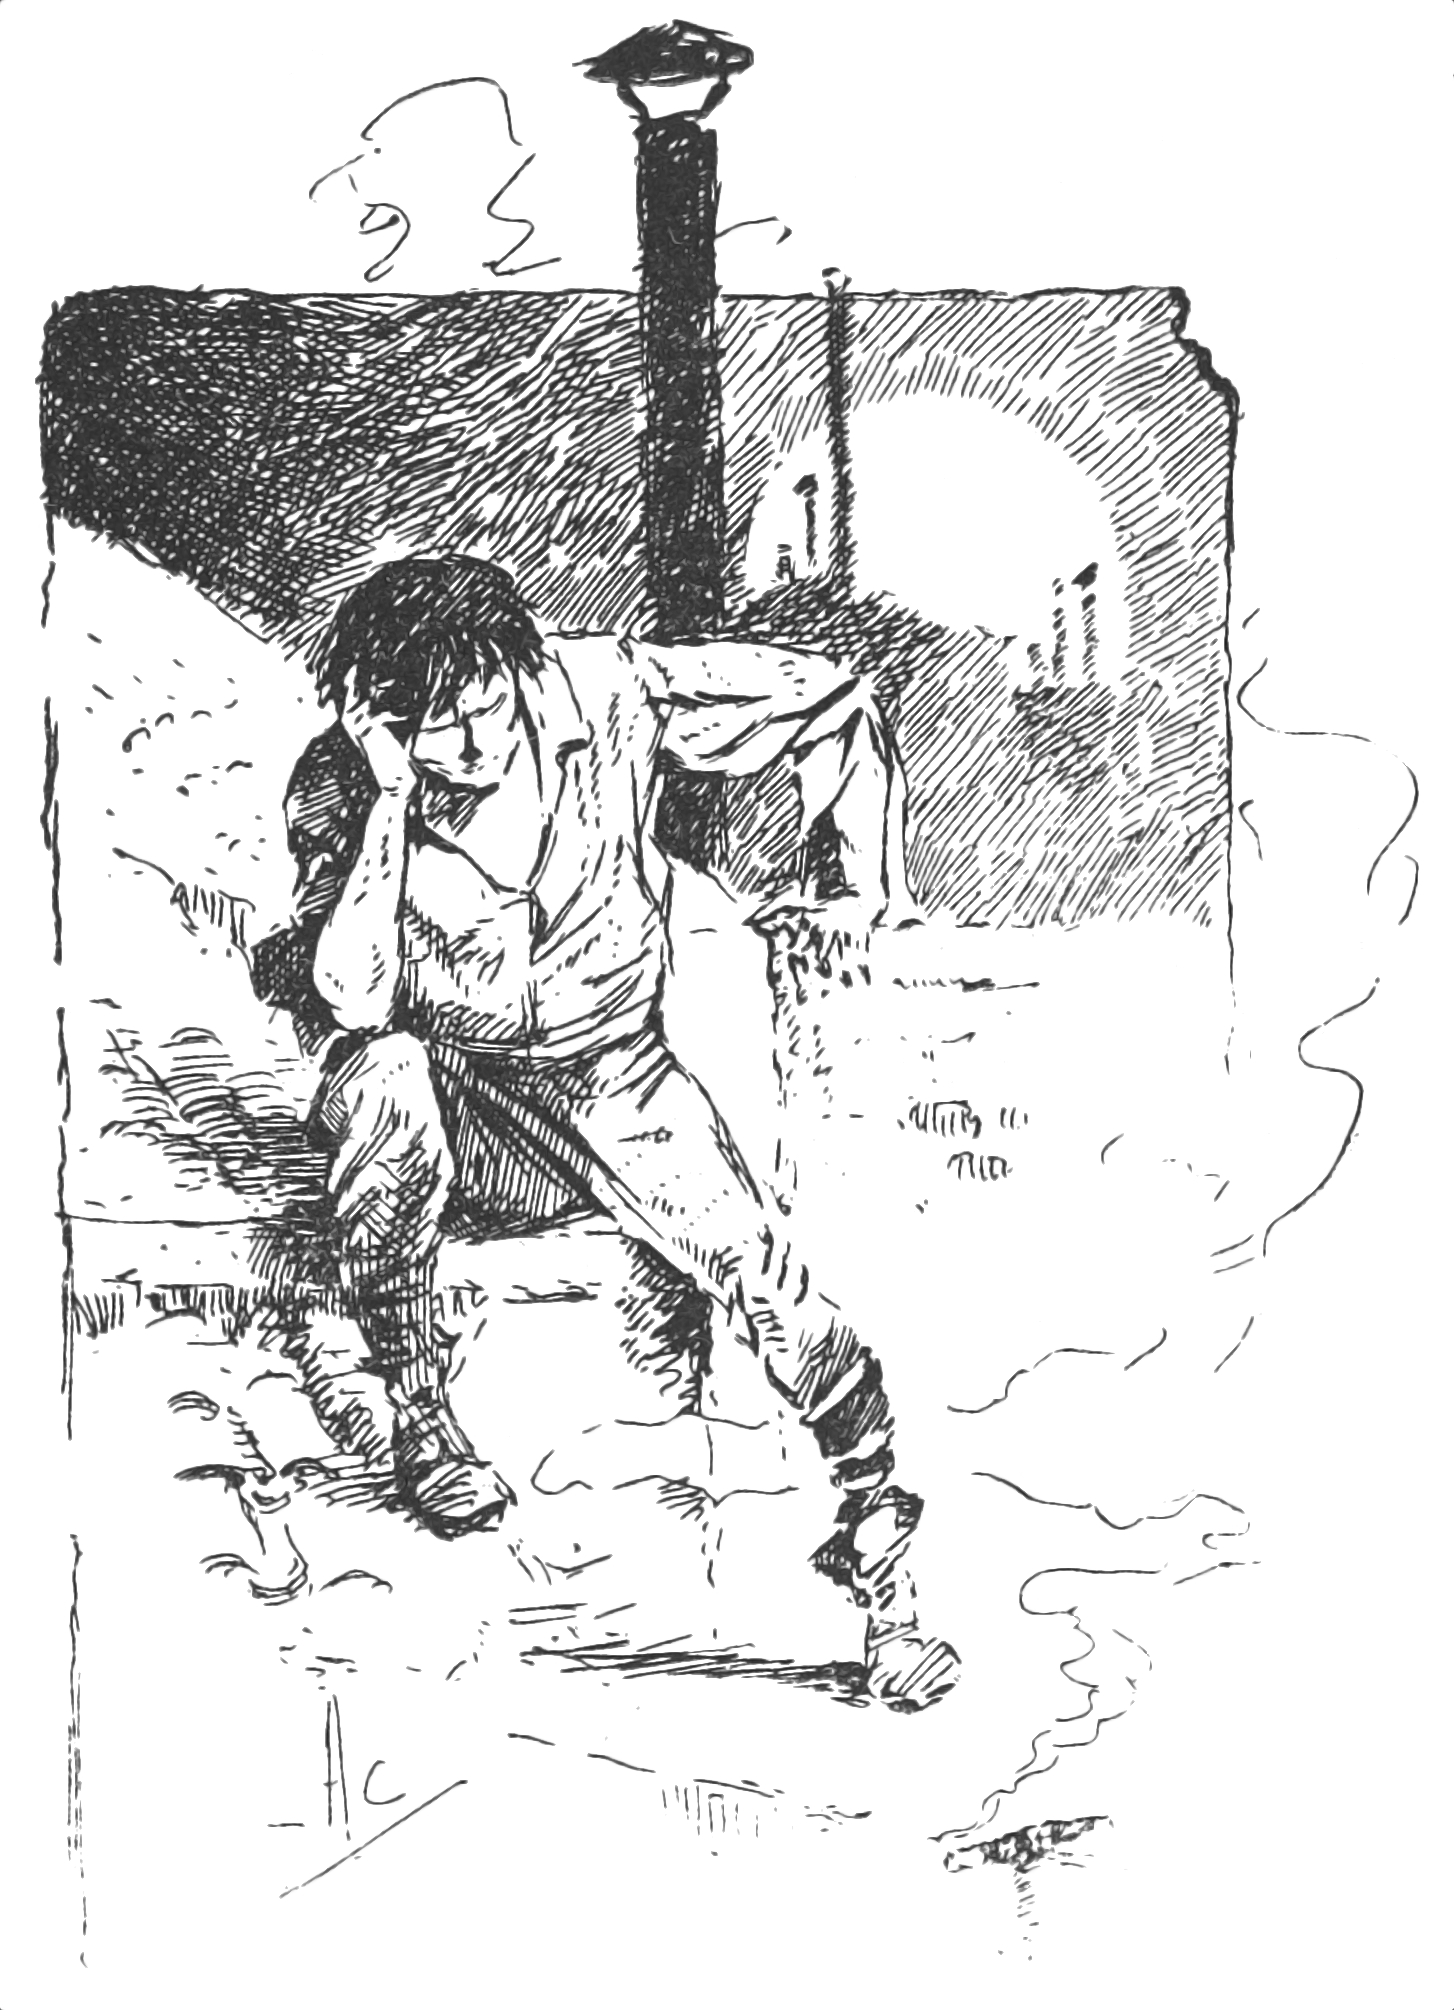
\includegraphics[width=0.6\textwidth]{24tailpiece}};
	\end{tikzpicture}
	

\end{a4}

\begin{letter}
	
	\begin{tikzpicture}[remember picture, overlay]  
		\node (tailpiece) at ($(current page.south)+(0cm,5cm)$) {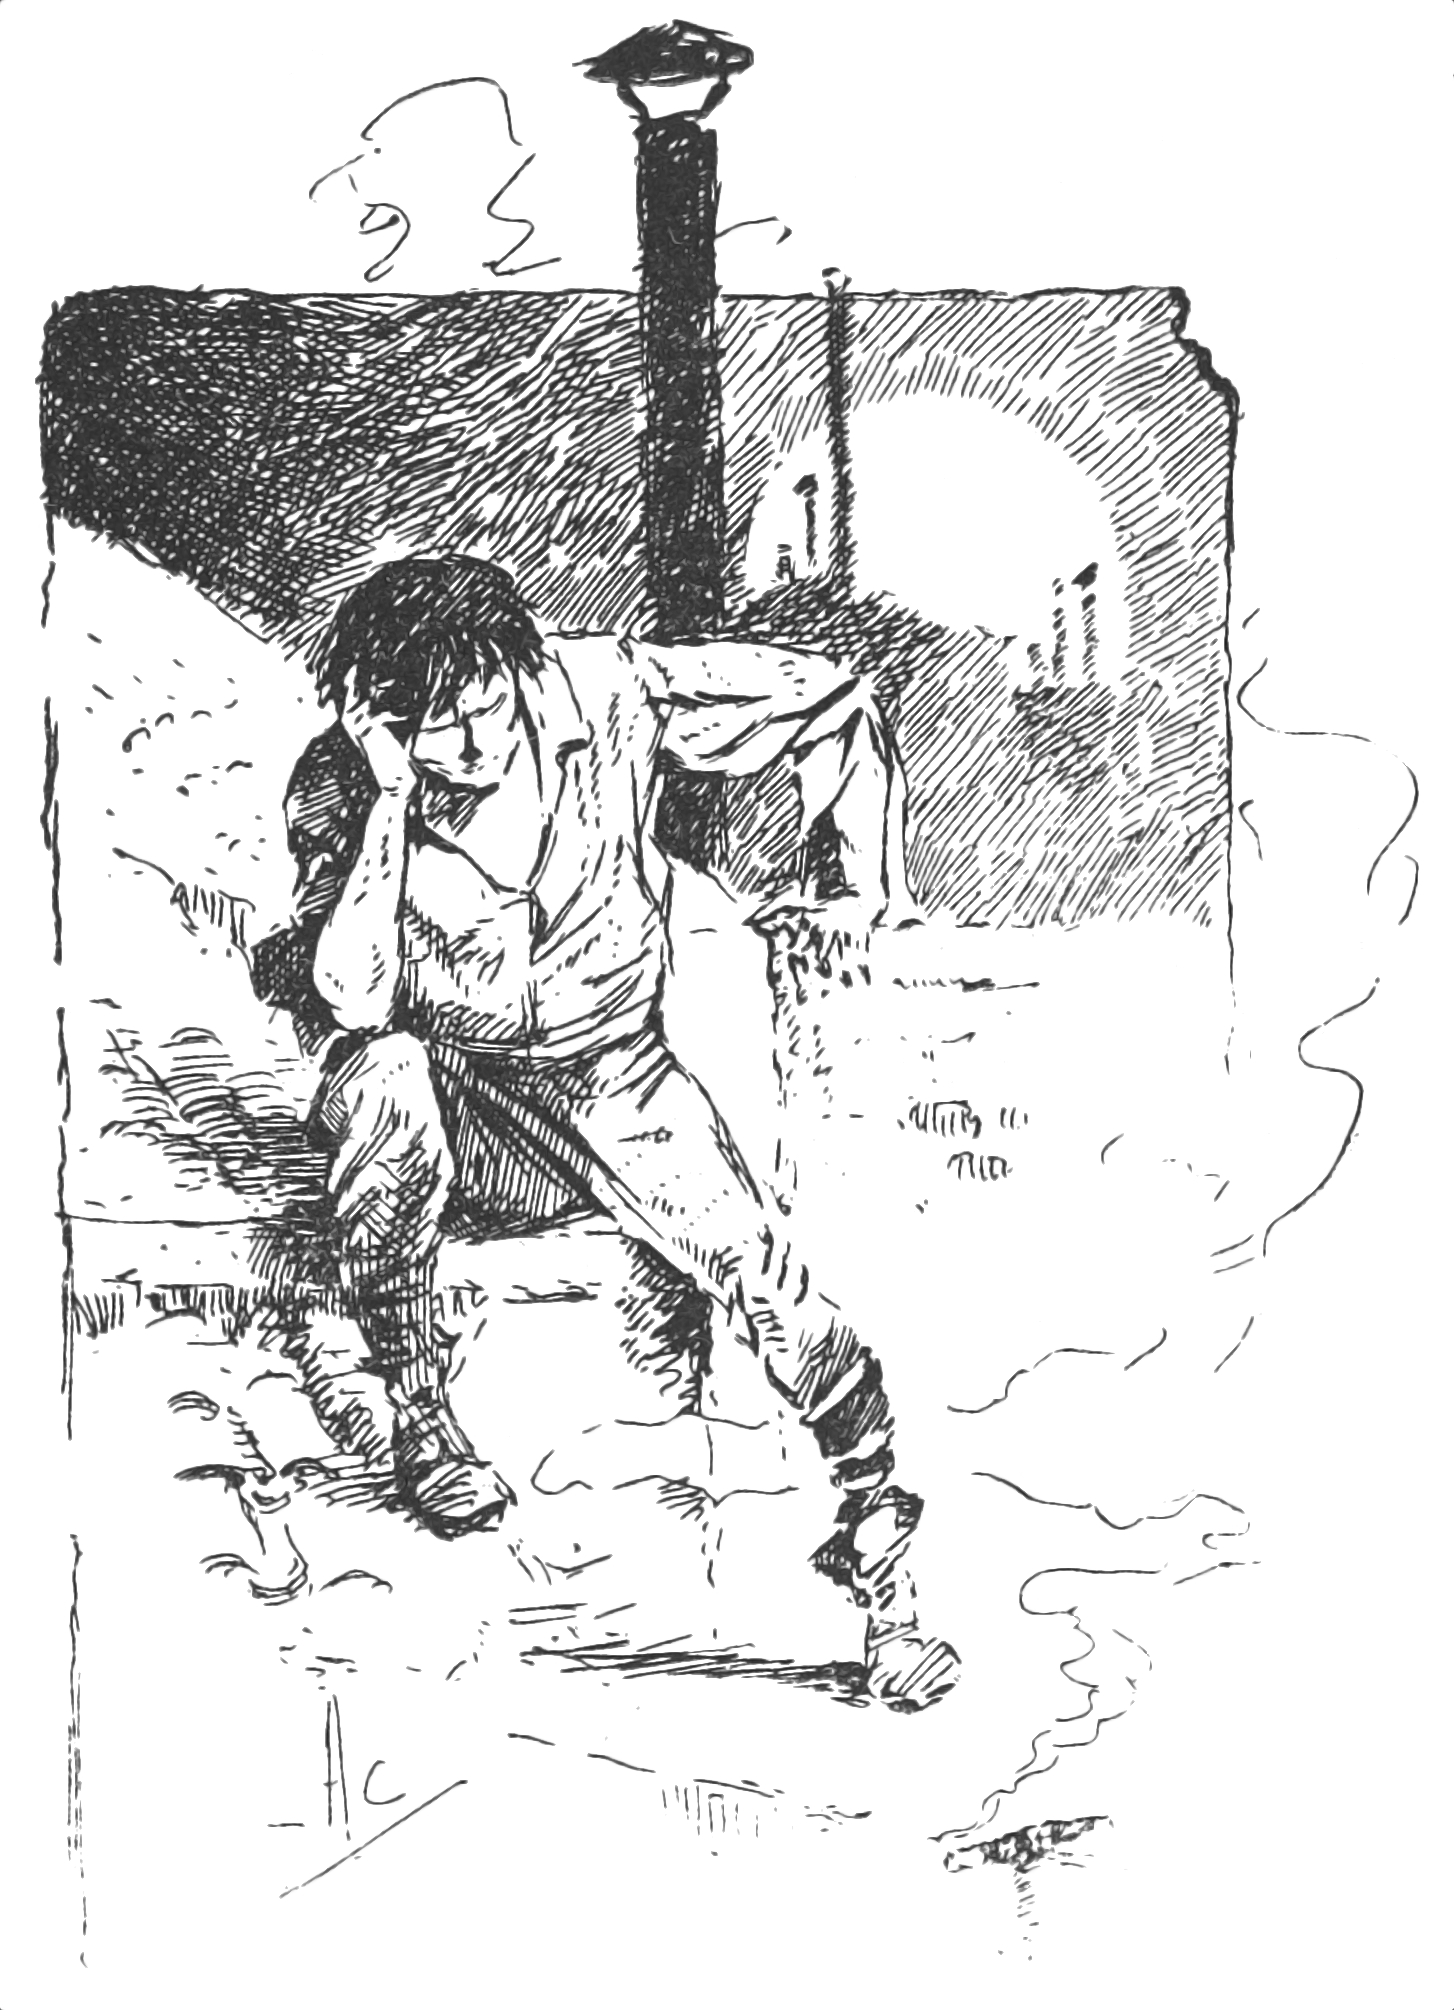
\includegraphics[width=0.4\textwidth]{24tailpiece}};
	\end{tikzpicture}

\end{letter}